\section{High Latitude Input}\label{cap:high_lat}
%
\subsection{Weimer}
%
To use the high latitude potential as defined by
Weimer the flag \flags{POTENTIAL\_MODEL = WEIMER} in the input file of a TIEGCM 
has to be set. The Weimer high latitude potential was not working to estimate 
the convection radius under Bz positive conditions in version 1.7 and 1.8 of TIEGCM.  
Additional problems concerning the crossover between the high latitude electric 
fields and the calculated dynamo fields for active conditions with relatively large 
convection radii theta0 were finally fixed in version 1.94 with the replacement of 
the constant cross-over co-latitudes with dynamic cross-over co-latitudes described 
in section \ref{cap:dynamic_cross_over_colat}.
%
\subsection{Heelis}
%
At high latitude the electric potential pattern can be prescribed as
determined by Heelis. The calculation of the
electric potential due to Heelis is not described since we didn't work
on this part of the code. The Heelis potential pattern is the
default if the flag \flags{POTENTIAL\_MODEL} is not specified. 
The Heelis model is also the
basis for the high latitude modifications described in the following
sections. Therefore when using these modifications the flag  
\flags{POTENTIAL\_MODEL = HEELIS} should be set in the input file.
%
\subsection{Dynamics cross-over co-latitudes} \label{cap:dynamic_cross_over_colat}
%
The TIEGCM uses an imposed electric field model such as the Weimer (2005) \cite{Weimer2005} or 
Heelis (1982) \cite{heelis1982} electric potential models at high magnetic latitudes above a 
critical magnetic co-latitude called \code{crit(1)}.  This is set at 15 degrees 
co-latitude, or at 75 geomagnetic latitude.  Below a second magnetic co-latitude called
\code{crit(2)}, 
the dynamo model calculates the electric field in the TIEGCM.  This is set at 30 
degrees co-latitude, or at 60 geomagnetic latitude.  Between 60 and 75 geomagnetic
latitude, there is a linear 
variation of the combined dynamo solution and the imposed high latitude solution.   
\flags{Crit} is set as a real parameter in \src{cons.F} \index{cons.F}. \\

The convection radius increases as a function of magnetic activity, and is offset 
towards 0 MLT from the magnetic pole by 1.1 degree for the Heelis (1982) \cite{heelis1982} convection 
model, and by 4.2 degrees for the Weimer (2005) \cite{Weimer2005} convection model.  Assuming the 
convection is centered on the magnetic pole, the following figure \ref{fig:convec_radius_Heelis} shows how the 
convection radius increases for the Heelis model in the TIEGCM as a function of Kp 
and also plots \code{crit(1)} and \code{crit(2)} lines.  The red dashed lines are the present 
constant crit(1) and crit(2) values, while the dashed green lines are the proposed 
'dynamic' crit(1) and crit(2) values.  The dynamic values are always equatorwards of 
the radius of convection, where crit(1) is set to be 5 degrees larger than the 
convection radius and crit(2) is 15 degrees larger.  This distance from the 
convection radius is actually a function of MLT because of the offset of the 
convection pattern towards 0 MLT. \\

%
\begin{figure}
  \centering
  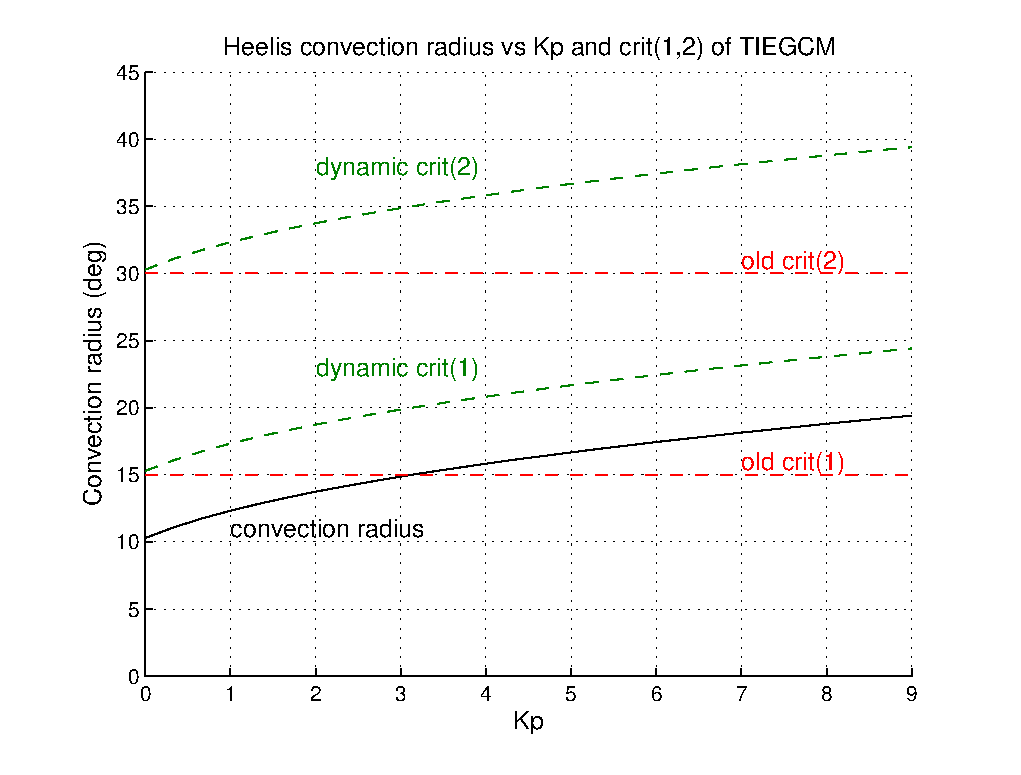
\includegraphics[scale=0.7]{./tex_plot/crad_kp_may11.eps}
  \caption{Heelis convection radius over Kp}
   \label{fig:convec_radius_Heelis}
\end{figure}
%
The Heelis convection radius maximizes at 19 degrees for Kp 9, and thus is never more than 
5 degrees equatorwards of the constant crit(1) and crit(2) values from the 4 degrees at Kp 9 
(19-15=4) and the additional 1.1 degrees offset towards 0 MLT.  However, the Weimer (2005) 
convection radius is approximately 20-25 degrees in active periods, and with the additional 
4.2 degree offset towards 0 MLT can be ~10-15 degrees equatorwards of the constant crit(1) at 
0 MLT, which is at the location of crit(2) and the dynamo only solution.  We found insufficient 
TEC magnitudes for 06348 between 16-22 UT using the constant crit values and Weimer (2005) 
potential patterns driven by 5-min IMF, but good TEC magnitudes when using dynamic crit values.  
Other tests showed NmF2 values on active days are generally improved in both the Weimer (2005) 
and Heelis (1982) convection cases using dynamic crit values.  \\

However, we have not finished our testing, especially since the Heelis NmF2 improved for all 
stations except the station closest to the crit(2) value for the WHI 
(Whole Heliosphere Interval: March 20, 2008 to April 16, 2008 - Solar Carrington Rotation 2068) 
period.  
Thus we have some more testing to determine where we should best place the dynamic crit values 
with respect to the convection radius and to each other.
%
\subsection{Modification of the high latitude input}
%
In the electrodynamo equation (\ref{eq:edyn}) we neglected so far the
 current part $J_{Mr}$ between the ionosphere and magnetosphere. The current
from the magnetosphere can be influenced by the electric field
distribution, however the mechanism is not fully understood. The total field-aligned
current between ionosphere and magnetosphere can be described as the divergence
of a magnetospheric current $\mathbf{K}^M$
%
\begin{equation}
   {J}_{Mr}  = \frac{1}{R_0 cos \lambda_m} \bigl(
    \frac{\partial K_{\phi}^M}{\partial \phi_m} + 
    \frac{\partial K_{|\lambda|}^M cos \lambda_m}{\partial | \lambda_m| } \bigr) 
    \label{eq:magcurrent}
\end{equation}
%
The height integrated current density $\mathbf{K}^M$ doesn't have 
to be realistic, but the divergence, i.e. the current $J_{Mr}$,
should be. Using the divergence assures that the integrated field-aligned
current over both hemispheres vanishes, and therefore there is no net current into the
ionosphere. The two components of the field-aligned
current $K_{\phi}^M$ and $K_{|\lambda|}^M$, eastward and poleward/ upward, 
can be differently defined depending on the acting region and the
mimicking mechanism. The different contributions 
are described in the following three subsections. Note that in the
default code non of these options is used. To use them one or all
of the flags
\flags{mod\_heelis}, \flags{J\_rR} and \flags{eqMgCnd} have to be set to 
\src{.true.} in the  \src{dynamo\_module}.
%.
\subsubsection{Field--aligned current}\label{cap:fldalg_curr}
%
This part has not been tested yet, however the source code can be found in 
\src{subroutine calrhs\_jrr}. To use the field--aligned part 
the flag  \src{J\_rR = .true.} 
in  \src{dynamo\_module} has to be set. 
The magnetospheric current components $K_{\phi}^M$ and 
$K_{|\lambda|}^M$ for the field--aligned current can be derived 
from a reference potential 
$\Phi_R$ which we assume is the Heelis potential for now. Using the
Heelis potential leads to realistic magnitudes and directions 
in the current, but
might not represent correctly the field-aligned current in the region 1.
%
\begin{align}
  K_{\phi}^M       &=  \frac{1}{R_0} \bigl( \frac{\Sigma_{\phi \phi}^T}{cos
   \lambda_m} \frac{\partial \Phi_R}{\partial \phi_m} + 
   \Sigma_{\phi \lambda}^T \frac{\partial \Phi_R}{\partial |\lambda_m|} \bigr) \label{eq:fac_phi}\\
  K_{|\lambda|}^M  &= \frac{1}{R_0 cos \lambda_m} \bigl( \Sigma_{\lambda \phi}^T
    \frac{\partial \Phi_R}{\partial \phi_m} + 
   \Sigma_{\lambda \lambda}^T cos \lambda_m 
   \frac{\partial \Phi_R}{\partial |\lambda_m|} \bigr) \label{eq:fac_lam}
\end{align}
%
%The factor $f_{\lambda}$ is set such that it's 1 poleward of the crit(1)
%$ \lambda_m^{crb}$ and zero equatorward. Thus, the current 
%represents region 1 current and is zero in the region 2.
%
%\begin{align}
%  f_{\lambda} = 1 \quad \text{for} \quad |\lambda_m| \ge  \lambda_m^{crb} \\ 
%  f_{\lambda} = 0 \quad \text{for} \quad |\lambda_m| <  \lambda_m^{crb} 
%\end{align}
%
%In TIEGCM the value for the convection reversal boundary $ \lambda_m^{crb}$  
%is set to $75^o$ in the
%\src{module cons}. Note that this is not a physical meaningful value since 
%the convection reversal boundary is fixed.
%For the modified reference potential in section \ref{cap:modrefpot} 
%a variable value for the convection reversal boundary will
%be used which is set in the \src{aurora module}. 

The current components in equations (\ref{eq:fac_phi}) and (\ref{eq:fac_lam})
are calculated in a similar way as the left hand side of the electrodynamo 
equation, which is described in section
\ref{chap:finitediff}. The conductance expressions in equation 
(\ref{eq:sig_dif1})--(\ref{eq:sig_dif4}) are used to calculate the current 
components in equations (\ref{eq:fac_phi}) and (\ref{eq:fac_lam}), and therefore
these conductances are input to the 
\src{subroutine calrhs\_jrr} where the current components eq. 
(\ref{eq:sig_dif1})--(\ref{eq:sig_dif4}) are calculated. 
The finite difference stencil for the partial derivatives in equations 
(\ref{eq:fac_phi}) and (\ref{eq:fac_lam})  is set up in  
\src{subroutine nsstencil}. In comparison to the set up of the finite difference 
stencil in section
\ref{chap:finitediff} for the left hand side of the electrodynamo equation, 
here, it's done for both hemispheres and 
without upwinding technique. Once the finite difference stencil is calculated 
the electric
potential $\Phi_R$ is inserted, which is done in \src{subroutine insert\_pot}, 
to calculate the
current components. Although the calculation is done for both hemisphere, 
it is not necessary since the used Heelis potential
is symmetric about the equator and the coefficients of the conductances in equations 
(\ref{eq:sig_dif1})--(\ref{eq:sig_dif4}) are already the sum of the two
hemispheres. After calculating the current it is added to the right hand side of the
electrodynamo equation (\ref{eq:edyn}).
%
\subsubsection{Equivalent magnetospheric conductances}\label{cap:magncond}
%
The magnetospheric field-aligned current can be influenced by the electric field
distribution in the ionosphere, and therefore depend on the electric potential. The
region 2 current with the shielding effect of strong electric fields from high to low
latitude is an example of this magnetosphere--ionosphere interaction. The region 2
current can be approximated by a Hall conductor. In addition, the 
magnetospheric ion loss
can be simulated by adding a zonal Pedersen conductance. 
In TIEGCM we adopt the concept from
\cite{peym93} by using equivalent magnetospheric conductances 
$\Sigma_{\phi \phi}^M$ and $\Sigma_{H}^M$. 
The magnetospheric current in eq. (\ref{eq:magcurrent}) can
be replaced by
%
\begin{align}
  K_{\phi}^M       &=  \frac{-1}{R_0} \bigl( \frac{\Sigma_{\phi \phi}^M}{cos
   \lambda_m} \frac{\partial \Phi}{\partial \phi_m} + 
   \Sigma_{H}^M \frac{\partial \Phi}{\partial |\lambda_m|} \bigr)  \label{eq:mageqcur_phi}\\
  K_{|\lambda|}^M  &=   \frac{\Sigma_{H}^M}{R_0 cos \lambda_m}
    \frac{ \partial \Phi_R}{\partial \phi_m} \label{eq:mageqcur_lam}
\end{align}
%
with $\Sigma_{\phi \phi}^M$ and $\Sigma_{H}^M$ being the equivalent magnetospheric zonal
Pedersen and Hall conductances. The values of $\Sigma_{\phi \phi}^M$ and $\Sigma_{H}^M$
are taken from figure 4 in \cite{peym93} and plotted in figure \ref{fig:magcond}. In 
\src{subroutine set\_cicr} the equivalent magnetospheric conductances 
are set up and added to the conductances due to solar ionization and
particle precipitation in \src{subroutine add\_cicr}. In figure 
\ref{fig:magcond} the equivalent magnetospheric
conductances start at $72^o$ magnetic latitude which is the 
convection reversal boundary for this specific
case. However, the convection reversal boundary varies with the geomagnetic conditions
and the location is determined in the \src{aurora module}. 
The contributions to the electrodynamo equation 
due to the equivalent magnetospheric conductances 
 are calculated in a similar way as
described in section \ref{cap:fieldlineintg} for the left hand side of the electrodynamo
equation. The conductances are calculated on the irregular spaced grid $\lambda_m^*$, 
but for the finite differencing the regular grid $\lambda_0$ in
 $\lambda_m^*$ is used. Therefore, the
difference in the partial derivatives due to the change from  $\lambda_m^*$ to  $\lambda_0$ 
have to be taken into account,
as described in table 
\ref{tab:transf_quantities}. The conductance quantities are then
 prepared for the finite differencing as shown in eq. 
(\ref{eq:sig_dif1}) and (\ref{eq:sig_dif3}) and added to the conductances due to solar
ionization and particle precipitation. To use the equivalent magnetospheric
conductances, the flag \flags{eqMgCnd} has to be set to 
\src{.true.} in the  \src{dynamo\_module}. 
%
\begin{figure}
  \centering
  \includegraphics[scale=0.3, angle=-90]{./tex_plot/magcond.epsi}
  \caption{Latitudinal variation of equivalent magnetospheric conductances 
    $\Sigma_{\phi \phi}^M$ ($C_r$) and $\Sigma_{H}^M$ ($C_i$) for the 
    convection reversal boundary at $72^o$.}
   \label{fig:magcond}
\end{figure}
%
\subsubsection{Modified reference potential}   \label{cap:modrefpot}
%
In the region 1 the magnetospheric current in eq.(\ref{eq:magcurrent}) can be represented
by the combination of a field--aligned current described in 
section \ref{cap:fldalg_curr} and a reference electric potential 
distribution $\Phi^R$. The later is described in
the following. The contribution to the magnetospheric current from a reference potential
can be specified by
%
\begin{align}
  K_{\phi}^M       &=  \frac{\Sigma^R}{R_0 cos
   \lambda_m} \frac{\partial (\Phi^R - \Phi)}{\partial \phi_m} \label{eq:refpotphi}\\
  K_{|\lambda|}^M  &=   \frac{\Sigma^R}{R_0 }
    \frac{\partial (\Phi^R - \Phi) }{\partial \phi_m} \label{eq:refpotlam}
\end{align}
%
The reference conductance $\Sigma^R$ is not a physical conductance, but determines how
strongly the calculated electric potential $\Phi$ reflects the reference potential
$\Phi^R$. The reference conductance is set to
%
\begin{align}
  \Sigma^R =& \text{min} \; \bigl( {\Sigma_{max}^R,\Sigma_b [ e^{|\lambda_m-\lambda_{crb}|
          \frac{2}{\alpha_t}}-1]}  \bigr) \quad \text{for} \quad |\lambda_m|
	   \ge  \lambda_m^{crb} \label{eq:sigmar1}\\ 
  \Sigma^R =& 0 \quad \text{for} \quad |\lambda_m| <  \lambda_m^{crb} \label{eq:sigmar2}
\end{align}
%
with $\alpha_t$ being the width of the transition zone, here $3^o$, equatorward of the
convection reversal boundary $\lambda_m^{crb}$. 
The maximum reference conductance 
$\Sigma_{max}^R$ is set to $10,000 \; S$ and the base conductance $\Sigma_b$ 
is 5 S. In the
polar cap region the electric potential should be the reference potential. In the source
code the Heelis potential is used for the reference
potential $\Phi^R$. The convection reversal boundary is denoted by $\lambda_m^{crb}$, 
which varies with the geomagnetic conditions, and is set in the \src{aurora module}.
In figure \ref{fig:sigma_r} the latitudinal variation of the
reference conductance $\Sigma^R$ is shown for $\lambda_m^{crb} = 72^o$. 
\\

In the source code the calling tree is the
following
%
\begin{verbatim}
subroutine dynamo
...
if (mod_heelis) then
   if(istep = 1 ) then call set_zigmar
   call add_zigmar
   call diff_rimr
   call add_rimr
endif
...
\end{verbatim}
%
To use the modified reference potential the flag 
\flags{mod\_heelis} in the  \src{dynamo\_module} has to be set to \src{.true.}. 
The current in the equations (\ref{eq:refpotphi}) and (\ref{eq:refpotlam})
are calculated like the left hand side of the electrodynamo equation 
which is described in section
\ref{chap:finitediff}. The reference conductances 
$\Sigma^R$ are calculated according to eq. (\ref{eq:sigmar1}) and 
(\ref{eq:sigmar2}) in \src{subroutine set\_zigmar}. 
The coefficients of the reference conductance are added 
in \src{subroutine add\_zigmar} to the conductances 
$\Sigma_{\phi \phi}$ and $\Sigma_{\lambda \lambda}$ of the electrodynamo equation.
The finite difference stencil is set up in
\src{subroutine diff\_rimr} by
\src{subroutine nsstencil}. In comparison to the set up of the stencil for 
the left hand side of the electrodynamo equation, in section
\ref{chap:finitediff}, the stencil is calculated for both hemispheres and no
upwinding technique are used. Once the finite difference stencil is 
calculated the electric
potential $\Phi_R$ is inserted to calculate the additional 
current for the right hand side of the electrodynamo equation
in \src{subroutine insert\_pot}. Although the additional current
is determined  for both hemisphere separately,
this is not necessary since the reference  potential and the coefficients 
of $\Sigma^R$
are symmetric about the equator.
%
%
\begin{figure}
  \centering
  \includegraphics[scale=0.3, angle=-90]{./tex_plot/sigma_r.epsi}
  \caption{Latitudinal variation of reference conductance 
    $\Sigma^R$ for  $\lambda_m^{crb}= 72^o$  }
   \label{fig:sigma_r}
\end{figure}
%
%
